%
%                  Politecnico di Milano
%
%        Students: Caravano Andrea, Cantele Alberto, Cancelliere Biagio
%            A.Y.: 2024/2025
%
%   Last modified: 05/05/2025
%
%     Description: Kratos 2: an all-in-one C development companion
%

\documentclass[aspectratio=1610,10.5pt]{beamer} % Beamer (presentazione, con font a dimensione 10.5 e aspect ratio 16:10)

\usepackage[T1]{fontenc} % codifica dei font
\usepackage[utf8]{inputenc} % lettere accentate da tastiera
\usepackage[english]{babel} % lingua del documento
\usepackage{lipsum} % genera testo fittizio
\usepackage{url} % per scrivere gli indirizzi Internet e/o di riferimento nella pagina

% \usetheme{Frankfurt} % tema 1

% \usetheme{Boadilla} % tema 2

\usetheme{Darmstadt} % tema 3

% \usecolortheme{default} % tema colori 1 (default)

\usecolortheme{rose} % tema colori 2

% \usecolortheme{whale} % tema colori 3

\setbeamersize{text margin left=5mm, text margin right=5mm} % margine di pagina

\setbeamertemplate{headline}{} % rimuove la barra di navigazione dall'intestazione
\setbeamertemplate{footline}[frame number] % numero di pagina in piè di pagina
\setbeamertemplate{navigation symbols}{} % rimuove simboli di navigazione
\setbeamercovered{invisible} % blocchi ancora da mostrare invisibili, esiste anche transparent

\usepackage{hyperref} % per modificare il comportamento dei collegamenti ipertestuali

\usepackage{graphicx} % per inserire immagini

\usepackage{blkarray} % per inserire blocchi Beamer

\usepackage{tikz} % pacchetto per la produzione di diagrammi
\usetikzlibrary{automata, positioning, arrows} % librerie per il tracciamento di ASF/FSM

\usepackage{minted} % per colorazione automatica del codice (installare pygments da Homebrew)
% \usepackage{pythonhighlight} % per Python

\usepackage{lmodern} % carattere macchina da scrivere (typewriter) con caratteri grassetti

\hypersetup{ % metadati di titolo e autore nel PDF
    hidelinks, % leva colore attorno collegamenti ipertestuali
    pdftitle={Kratos 2: an all-in-one C development companion},
    pdfauthor={Andrea Caravano - Alberto Cantele - Biagio Cancelliere}
}

\begin{document}
% Pagina del titolo
\title{\textbf{Kratos 2: an all-in-one C development companion}}
\author{A.A. 2024/25\\Andrea Caravano\and Alberto Cantele\and Biagio Cancelliere}
%\institute{Politecnico di Milano}
\date{May 9, 2025}
\titlegraphic{
\includegraphics[height=%
0.15\textheight]{../res/logo-polimi}}

% logo in basso a destra
%\logo{\includegraphics[height=%
%0.15\textheight]{logo}}

% Creazione pagina del titolo
\begin{frame}
    \titlepage
\end{frame}

% indice del documento (relativo alle sezioni e non ai frame)
\begin{frame}{Agenda}
    \tableofcontents
\end{frame}

\logo{} % rimuove il logo dalle slide successive

\section{Kratos 2: a brief introduction}
\begin{frame}{Kratos 2: a brief introduction}
    \begin{center}
        
\includegraphics[height=%
        0.15\textheight]{../res/logo-kratos}
    \end{center}

    \textbf{Kratos 2} is a formal verification tool for \textbf{imperative programs}, mostly aimed at C projects.

    \smallskip

    It translates code into an intermediate verification language called \textbf{K2}, specifically designed for Kratos, which has a \textbf{formal semantics, mimicking the Assembly language}.

    \smallskip

    It embeds precise checking of both \textbf{safety} (e.g., no assertion failure) and \textbf{liveness} properties (e.g., eventual termination), through \textbf{assertions}.
\end{frame}

\begin{frame}{Main functionalities}
    Kratos 2 integrates state-of-the-art \textbf{SAT/SMT solvers} and supports \textbf{symbolic execution}, \textbf{counterexample generation}, and \textbf{interactive simulation}.

    \medskip

    It provides a \textbf{customizable C front-end}, a flexible \textbf{Python API} and can translate verification tasks into multiple low-level formalisms, for easy integration into development pipelines.

    \medskip

    C programs can be \textbf{directly translated into the intermediate language K2} via a complete translator, implemented in Python.

    \bigskip

    Kratos' main engines have been developed with verification of \textbf{low-level software} in mind, like system modules or bit-manipulation computations.
\end{frame}

\begin{frame}[fragile]{Running configurations}
    A Kratos \textbf{running configuration} is composed of a set of \textbf{inter-dependent} stages:

    \begin{block}{Stages}
        \begin{itemize}
            \item \texttt{cex}: cex trace reconstruction.
            \item \texttt{cfg}: CFG building.
            \item \texttt{check\_inv}: check given inductive invariant.
            \item \texttt{flatten}: flattening of expressions.
            \item \texttt{inline}: function inlining.
            \item \texttt{mc}: model checking.
            \item \texttt{parse}: input file parsing.
            \item \texttt{sim}: interactive simulation.
            \item \texttt{smt}: use Kratos as an SMT solver (MathSAT).
            \item \texttt{symexec}: perform symbolic execution.
            \item \texttt{trans}: transition system encoding.
        \end{itemize}
    \end{block}

    Intermediate computations can be dumped, but they are mostly in a \textbf{proprietary format}.
\end{frame}

\begin{frame}{Overall architecture}
    \begin{center}
        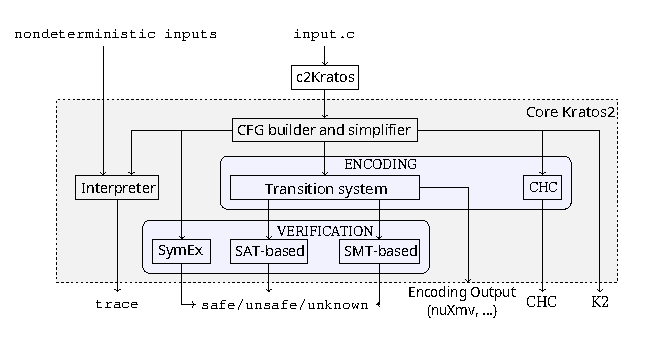
\includegraphics[height=%
        0.85\textheight]{../res/architecture-paper}
    \end{center}
\end{frame}

\begin{frame}{Distribution and installation}
    It is distributed by \textsc{Fondazione Bruno Kessler} (Trento, Italy) as a \textbf{closed-source, pre-compiled} binary for both \textbf{Linux} and \textbf{Windows}, only on \texttt{x64} architecture.

    Currently, the latest version publicly available is version \texttt{2.2}.

    \begin{center}
        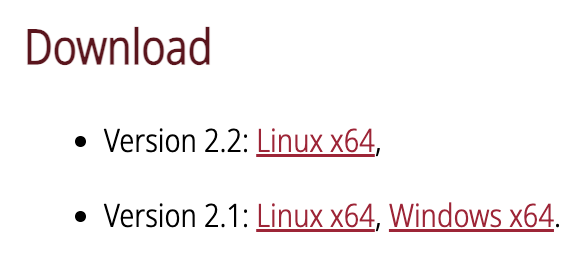
\includegraphics[height=%
        0.25\textheight]{../res/download-kratos}
    \end{center}

    Kratos 2 \textbf{does not require installation} on the system, being distributed as a \textbf{complete binary}, carrying most of the dependencies needed to run on modern operating systems.

    \smallskip

    The tool is \textbf{not distributed for neither macOS nor ARM-based chips}: a \textsc{Docker} container (as part of a \textsc{development container}) or a Virtual Machine are the most reasonable choices in which running Kratos, in those cases.
\end{frame}

\begin{frame}[fragile]{A sketched Docker container providing Kratos} % il frame va impostato come fragile per minted
    \begin{block}{\textsc{Dockerfile}}
        % dimensione di font per minted, altra possibilità small
            \begin{minted}[fontsize=\footnotesize]{text}
# Python's Debian-based image
FROM --platform=linux/amd64 python:3.11-bookworm
# Python 3.11 is the maximum supported version for C2Kratos

#### PYTHON DEPENDENCIES (for the C to Kratos conversion tool) ####
RUN pip install pycparser pcpp

#### STANDARD C DEVELOPMENT TOOLCHAIN ####
RUN apt update \ # upgrade and environment setup omitted...
    && apt install gdb hotspot valgrind build-essential cmake nano curl tar gzip

#### DOWNLOAD KRATOS2 ####
ARG KRATOS_RELEASE=https://kratos.fbk.eu/releases/kratos-2.2-linux64.tar.gz
ARG DESTINATION_FOLDER=kratos-2.2-linux64

RUN curl --output ./release ${KRATOS_RELEASE}

RUN tar -zxvf ./release
RUN mv ./${DESTINATION_FOLDER}/* /kratos

# Permissions, path, users and environment cleanup omitted...
            \end{minted}
    \end{block}
\end{frame}

\section{Model checking and SATisfiability: a theoretical overview}
\begin{frame}{Model checking}
    \textbf{Model checking} is an automated technique to verify whether a system (often modeled as a transition system) satisfies a given specification, typically expressed in temporal logic.

    \bigskip

    There are two main types of properties:
    \begin{itemize}
        \item \textbf{Safety properties}: assert that \textit{nothing bad ever happens} (e.g., a bad prefix).
        \item \textbf{Liveness properties}: assert that \textit{something good eventually happens} (e.g., every request eventually gets a response).
    \end{itemize}

    \medskip

    In Kratos, they are expressed as \textbf{program assertions} through \textit{labels}.
\end{frame}

\begin{frame}{SAT and SMT}
    \begin{itemize}
        \item \textbf{SAT (Boolean Satisfiability)} is the problem of deciding if a propositional logic formula can be made true by assigning truth values to its variables.

            \smallskip

            SAT solvers, like Kratos, are fast and widely used to verify purely boolean conditions.
        \item \textbf{SMT (Satisfiability Modulo Theories)} extends SAT by handling richer data types and \textbf{theories}:
            \begin{itemize}
                \item \textbf{Integers and real numbers}: Handling arithmetic operations and inequalities.
                \item \textbf{Arrays}: Reasoning about array properties, access, and updates.
                \item \textbf{Bit-vectors}: Working with fixed-width bit strings and bitwise operations.
                \item \textbf{Uninterpreted Functions}: Dealing with functions whose specific implementation is not known, but whose properties (like consistency) can still be reasoned about.
            \end{itemize}
    \end{itemize}
\end{frame}

\begin{frame}{SMT Solvers}
    \textbf{SMT solvers} (e.g., MathSAT, on which Kratos is based) are particulary well-suited for \textbf{software verification}. Programs often involve a mix of boolean logic and operation on various data types.

    SMT allows verification tool to reason about the complex interplay between these elements.

    \bigskip

    Tools like \textbf{Kratos 2} embed state-of-the-art SMT solvers, which enables them to:

    \smallskip

    \begin{itemize}
        \item \textbf{Verify properties of a program}: check for properties expressed as assertions by examining whether the negation of the property is satisfiable by any reachable state.
        \item \textbf{Perform symbolic execution}: explore all possible program paths without the need to run the program with concrete fixed inputs.
            Instead, they replace variables with symbolic values and maintain constraints on these values as the execution proceeds.
        \item \textbf{Generate counterexamples}: if a property is found to be violated, the SMT solver can often provide a concrete trace and assignment map of its variables, leading to the violation and showing a useful starting point for debugging purposes.
    \end{itemize}
\end{frame}

\begin{frame}[fragile]{Model checking in Kratos}
    Kratos implements three main model checking \textbf{algorithms}, with an eye on low-level software verification:
    \begin{itemize}
        \item \textbf{BMC}: standard Bounded Model Checking.
        \item \textbf{IC3}: the main algorithm used by Kratos, based on barriers.
        \item Symbolic model checking-based algorithms, using \textbf{mathematical induction}.
    \end{itemize}
    \begin{block}{Bounded Model Checking}
        BMC stems from the idea that a cycle occurs within a path of bounded length (number of states + 1): this helps with the detection of \textbf{back loops}, underlining infinite paths.

        \smallskip

        Given $k > 0$, we can encode the \textbf{unfolding} up to $k$ steps: suitable constraints are used to build a formula exhibiting a counterexample to the interested property of length at most $k$.
    \end{block}
\end{frame}

%    \begin{frame}{The K-induction and BMC algorithms}
%        \begin{block}{K-induction}
%            Inspired by mathematical induction: a base case shows invariant properties up to the $k$-th execution.

%            \smallskip

%            $I(s_0)\ \land\ T(s_0, s_1)\ \land\ \dots\ \land\ T(s_{k-1}, s_k) \implies P(s_0)\ \land\ P(s_1)\ \land\ \dots\ \land\ P(s_k)$

%            \smallskip

%            If $P(s_0)\ \land\ P(s_1)\ \land\ \dots\ \land\ P(s_{k-1})\ \land\ T(s_0, s_1)\ \land\ \dots\ \land\ T(s_k, s_{k+1}) \implies P(s_k)$
%        \end{block}
%    \end{frame}

\begin{frame}{The IC3 model checking algorithm: a sketch}
    \textbf{Incremental Construction of Inductive Clauses} (IC3) is a SAT-based model checking algorithm that aims at optimizing the number of inspected groups of states through \textbf{barriers}.

    \medskip

    At each step, the algorithm's evolution is described by \textbf{frames}: an inductive invariant.

    \begin{block}{Implementation sketch}
        \begin{itemize}
            \item Frame 0 ($F_0$) is built: the system's initial state collection.
            \item Frame 1 ($F_1$) is built: a transition step is performed (it must contain $F_0$).
            \item A set of constraints is formed and checked for: if, from $F_1$, a violating state in the group is reachable, we try to identify a descriptive clause ($c$).
            \item For violating constraints, the generalized explicit exclusion clause ($c$, \textbf{barrier}) is added to $F_1$.
            \item If the resulting frame is stable (no violations derive out of the generalization $\Rightarrow$ an invariant has been found), the new constraints are propagated and $F_2$ is built.
            \item Otherwise, a counterexample results from the contradiction of the initial states!
            \item The algorithm ends when
                $F_i = F_{i+1}$ (induction step: each transition stays in $F_i$).
        \end{itemize}
    \end{block}

    % Variants:
    % ABS (lazy abstraction): each frame F_i threats only a subset of variables as comnstraints, the others are threated as primary inputs. A counterexample is then refined sub-calling IC3.
    % K-ind: the induction step is shifted to k, so each frame is k-step apart.
    % Simplified: limits generalization to a unique iteration: faster but only simple clauses are produced (less robust).
    % extensions with SAT environment, CTG-based exploring less robust clauses but more efficient and BMC-based.
\end{frame}

\section{The Assembly-inspired intermediate language K2}

\begin{frame}[fragile]{Data types}
    K2 uses S-expression for its concrete syntax, representing structured data in textual format.
    \begin{block}{Basic Types}
            \begin{minted}[fontsize=\footnotesize]{text}
bool, int, real
            \end{minted}
    \end{block}
    \begin{block}{Bit-vectors}
            \begin{minted}[fontsize=\footnotesize]{text}
(sbv SIZE), (ubv SIZE)
            \end{minted}
    \end{block}
    \begin{block}{Floating-point numbers}
            \begin{minted}[fontsize=\footnotesize]{text}
(fp EXPONENT MANTISSA)
            \end{minted}
    \end{block}
    \begin{block}{Maps (arrays)}
            \begin{minted}[fontsize=\footnotesize]{text}
(map INDEX ELEM)
            \end{minted}
    \end{block}
    \begin{block}{Enumerations}
            \begin{minted}[fontsize=\footnotesize]{text}
(enum val1 val2 ...)
            \end{minted}
    \end{block}
\end{frame}

\begin{frame}[fragile]{Expressions and declarations}
    \begin{block}{Functions}
            \begin{minted}[fontsize=\footnotesize]{text}
(fun NAME (ARG_1 ...) (RET_1 ...))
            \end{minted}
    \end{block}
    \begin{block}{Variables}
            \begin{minted}[fontsize=\footnotesize]{text}
(var NAME TYPE)
            \end{minted}
    \end{block}
    \begin{block}{Constants}
            \begin{minted}[fontsize=\footnotesize]{text}
(const VALUE TYPE)
            \end{minted}
    \end{block}
    \begin{block}{Type conversions}
            \begin{minted}[fontsize=\footnotesize]{text}
(cast ...), (bitcast ...)
            \end{minted}
    \end{block}
    \begin{block}{Logical operations}
            \begin{minted}[fontsize=\footnotesize]{text}
and, or, not
            \end{minted}
    \end{block}
    \begin{block}{Arithmetic}
            \begin{minted}[fontsize=\footnotesize]{text}
add, sub, mul, div, rem
            \end{minted}
    \end{block}
\end{frame}

\begin{frame}[fragile]{Statements}
    \begin{block}{Bit-level operations}
            \begin{minted}[fontsize=\footnotesize]{text}
bitand, bitor, bitxor, bitnot, lshift, rshift
            \end{minted}
    \end{block}
    \begin{block}{Comparisons}
            \begin{minted}[fontsize=\footnotesize]{text}
eq, lt, le, gt, ge
            \end{minted}
    \end{block}
    \begin{block}{Maps}
            \begin{minted}[fontsize=\footnotesize]{text}
mapget, mapset
            \end{minted}
    \end{block}
    \begin{block}{Floating-point checking}
            \begin{minted}[fontsize=\footnotesize]{text}
isnan, isinf, etc.
            \end{minted}
    \end{block}
    \begin{block}{Assignments}
            \begin{minted}[fontsize=\footnotesize]{text}
(assign VAR EXPR)
            \end{minted}
    \end{block}
    \begin{block}{Assumptions}
            \begin{minted}[fontsize=\footnotesize]{text}
(assume EXPR)
            \end{minted}
    \end{block}
\end{frame}

\begin{frame}[fragile]{Statements}
    \begin{block}{Labels}
            \begin{minted}[fontsize=\footnotesize]{text}
(label NAME)
            \end{minted}
        Labels are heavily used for \textbf{model checking}, their usage will be further expanded later.
    \end{block}
    \begin{block}{Jumps (deterministic)}
            \begin{minted}[fontsize=\footnotesize]{text}
(jump TARGET)
            \end{minted}
    \end{block}
    \begin{block}{Jumps (conditionals)}
            \begin{minted}[fontsize=\footnotesize]{text}
(condjump COND TARGET)
            \end{minted}
    \end{block}
    \begin{block}{Sequential code block}
            \begin{minted}[fontsize=\footnotesize]{text}
(seq STMT1 STMT2 ...)
            \end{minted}
    \end{block}
    \begin{block}{Function call}
            \begin{minted}[fontsize=\footnotesize]{text}
(call FUNC ARGS RETS)
            \end{minted}
    \end{block}
\end{frame}

\begin{frame}[fragile]{Functions}
    \begin{block}{Function definition}
            \begin{minted}[fontsize=\footnotesize]{text}
(function NAME (PARAMS) (return RETS)
(locals VARS)
BODY)
            \end{minted}
    \end{block}
    \begin{itemize}
        \item  \textbf{NAME}: function identifier
        \item  \textbf{PARAMS, RETS}: input/return parameters
        \item  \textbf{VARS}: local variables
        \item  \textbf{BODY}: sequence of statements
    \end{itemize}
\end{frame}

\begin{frame}[fragile]{A full K2 program overview}
    \begin{block}{Program structure}
            \begin{minted}[fontsize=\footnotesize]{text}
(type TYPENAME TYPE)
(entry MAIN_FUNC)
(init CONSTRAINT)
(globals VARS)
FUNCTION_1
...
FUNCTION_N
            \end{minted}
    \end{block}
    \begin{itemize}
        \item  \textbf{TYPES}: aliases like type definitions
        \item  \textbf{ENTRY POINT}: main function
        \item  \textbf{INIT}: global state constraints
        \item  \textbf{GLOBALS}: declared global variables
    \end{itemize}
\end{frame}

\begin{frame}[fragile]{Assertions and verification properties}
    \begin{block}{Verification properties}
            \begin{minted}[fontsize=\footnotesize]{text}
(! SEXP :KEY VALUE)
            \end{minted}
    \end{block}
    \begin{itemize}
        \item  \textbf{(! LABEL :error NAME)}: this point is unreachable
        \item  \textbf{(! LABEL :live NAME)}: must be reachable infinitely often
        \item  \textbf{(! LABEL :notlive NAME)}: must eventually not be reached
    \end{itemize}
\end{frame}

\section{An introductory complete example: from C to Kratos}
\begin{frame}[fragile]{A first problem: an infinite loop}
    \begin{columns}
        \begin{column}{0.3\textwidth}
            \begin{block}{C implementation}
                    \begin{minted}[fontsize=\footnotesize]{C}
#include <assert.h>

int glbl = 0;

int f(int x) {
    if (glbl > 0) {
        return x - 1;
    } else {
        // our case
        glbl = 0;
        return x;
    }
}
                    \end{minted}
            \end{block}
        \end{column}
        \begin{column}{0.65\textwidth}
            \begin{block}{K2 translation}
                    \begin{minted}[fontsize=\footnotesize]{text}
(type cint (sbv 32))
(entry init_and_main)
(globals (var glbl cint))

(function f ((var x cint))
    (return (var ret cint)) (locals)
    (seq
        (jump (label then) (label else))
        (label then)
        (assume (op gt glbl (const 0 cint)))
        (assign ret (sub x (const 1 cint)))
        (jump (label end))
        (label else)
        (assume (op not (op gt glbl (const 0 cint))))
        (assign glbl (const 0 cint))
        (assign ret x)
        (label end)))
                    \end{minted}
            \end{block}
        \end{column}
    \end{columns}
\end{frame}

\begin{frame}[fragile]{A first problem: an infinite loop}
    \begin{columns}
        \begin{column}{0.35\textwidth}
            \begin{block}{C implementation}
                    \begin{minted}[fontsize=\footnotesize]{C}
void main(void) {
    int y;
    while (y > 0) {
        y = f(y);
    }

    // failure of the assertion
    // is an unreachable point!
    assert(glbl == 0);
}
                    \end{minted}
            \end{block}
        \end{column}
        \begin{column}{0.60\textwidth}
            \begin{block}{K2 translation}
                    \begin{minted}[fontsize=\footnotesize,escapeinside=||]{text}
(function main () (return) (locals (var y cint))
    (seq
        (label while)
        (jump (label inwhile) (label endwhile))
        (label inwhile)
        (assume (op gt y (const 0 cint)))
        (call f y y)
        (jump (label while))
        (label endwhile)
        (assume (op not (op gt y (const 0 cint))))
        (jump (label then) (label else))
        (label then)
        |\textbf{(assume (op not (op eq glbl (const 0 cint))))}|
        |\textbf{(! (label err) :error assert-fail)}|
        (label else)))

(function init_and_main () (return) (locals)
    (seq
        (assign glbl (const 0 cint))
        (call main)))
                    \end{minted}
            \end{block}
        \end{column}
    \end{columns}
\end{frame}

\begin{frame}[fragile]{A first problem: an infinite loop}
    Translation of C source code to the \textsc{K2} intermediate language is possible through the embedded \texttt{C2Kratos} translator, implemented as a \textsc{Python} project.

    \medskip

    Let's \textbf{translate} our example:

    \begin{block}{Linux shell command}
            \begin{minted}{bash}
python /kratos/tools/c2kratos.py ./example.c -o ./example.k2
            \end{minted}
    \end{block}

    \pause

    \bigskip

    Let's now apply \textbf{model checking} and confirm our intuition about the unreachability of the assertion failure condition, meaning the assertion cannot fail.

    \begin{block}{Linux shell command}
            \begin{minted}{bash}
kratos -stage=mc ./example.k2
            \end{minted}
    \end{block}
\end{frame}

\begin{frame}[fragile]{A first problem: an infinite loop}
    \begin{block}{Kratos output}
            \begin{minted}[fontsize=\footnotesize]{text}
parsing... done (0.024)
flattening... done (0.004)
inlining functions... done (0.004)
flattening after inlining... done (0.000)
building control-flow graph... done (0.004)
encoding into transition system... done (0.026)
Trans encoder statistics:
...
model checking...
checking property 0
...
model checking... done (0.081)

Model checker statistics:
  ...

Global statistics:
  total_time = 0.183
  memory_used_mb = 267

safe
            \end{minted}
    \end{block}
\end{frame}

\section{The Competition on Software Verification}

\begin{frame}{SV-COMP}
    \begin{center}
        
\includegraphics[height=%
        0.25\textheight]{../res/logo-svcomp}
    \end{center}

    \textbf{SV-COMP} (Competition on Software Verification) aims at \textbf{standardizing comparison} among software-verification tools, thanks to an established set of verification tasks.

    \bigskip

    It provides a \textbf{snapshot} of the state-of-the-art in the software verification community, providing benefit to students and researchers, \textbf{crediting} their development work.
\end{frame}

\begin{frame}[fragile]{Kratos 2 wrappers for SV-COMP}
    In its current state, Kratos' implementation is \textbf{heavily focused} on tackling and optimizing the resolution to the \textbf{verification tasks provided by SV-COMP}.

    \bigskip

    It provides specific declarations for SV-COMP specifications and a wrapper for automated benchmarking.

    \begin{block}{C2Kratos manual configuration}
            \begin{minted}{bash}
python /kratos/tools/c2kratos.py
    --svcomp --svcomp-spec properties/property.prp
        code.c | kratos -stage=mc [eventual options...]
            \end{minted}
    \end{block}

    \pause

    \begin{block}{Automated wrapper}
            \begin{minted}{bash}
python kratos-svcomp.py code.c
            \end{minted}
    \end{block}
\end{frame}

\begin{frame}{Results of a comparison}
    \begin{center}
        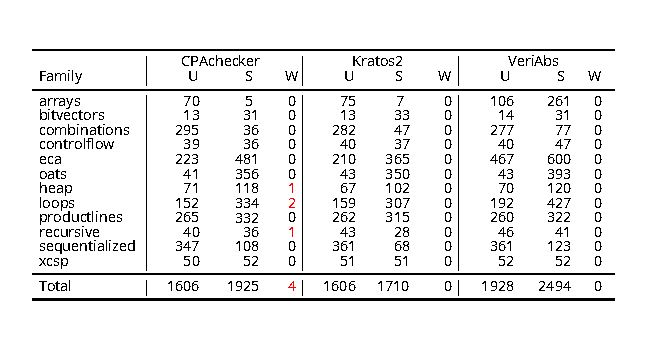
\includegraphics[height=%
        0.85\textheight]{../res/comparison-paper}
    \end{center}
\end{frame}

\section{An efficient modulo operation}

\begin{frame}{An efficient modulo operation}
    Let's consider \textbf{numbers in the form $2^{s}-1$}, with $s \in \mathbb{Z}^{+}$

    \medskip

    They represent, in binary notation, all combinations that are represented \textbf{only by ones}:

    \bigskip

    $s = 1 \Rightarrow 2^s-1 = 1_{10} = 1_2$

    \smallskip

    $s = 2 \Rightarrow 2^s-1 = 3_{10} = 11_2$

    \smallskip

    $s = 3 \Rightarrow 2^s-1 = 7_{10} = 111_2$

    \smallskip

    $s = 4 \Rightarrow 2^s-1 = 15_{10} = 1111_2$

    \smallskip

    $s = 5 \Rightarrow 2^s-1 = 31_{10} = 11111_2$

    \bigskip

    And so on\ldots
\end{frame}

\begin{frame}{An efficient modulo operation}
    Now, we would like to use these to \textbf{speed up the standard modulo operation} implementation.

    \bigskip

    $2^s = (2^s - 1) + 1 \implies 2^s\ mod\ (2^s - 1) = 1$

    \bigskip

    Modular arithmetic rules show that:

    \smallskip

    If $a\ mod\ n = b \Rightarrow a \equiv b\ (mod\ n)$, then $a^k = b^k\ (mod\ n)$ for $k \in \mathbb{Z}$

    \medskip

    So, the same rule applies also for higher orders!

    \smallskip

    $(2^s)^2\ mod\ (2^s - 1) = 1^2 = 1$

    \smallskip

    $(2^s)^3\ mod\ (2^s - 1) = 1^3 = 1$

    \smallskip

    $(2^s)^4\ mod\ (2^s - 1) = 1^4 = 1$

    \smallskip

    $(2^s)^5\ mod\ (2^s - 1) = 1^5 = 1$

    \bigskip

    And so on\ldots
\end{frame}

\begin{frame}{An efficient modulo operation}
    Let's remember how a number $n$ in base 10 is decomposed in powers of 2 (the same rule applied for conversions between the two basis):

    \bigskip

    $n = a_0 + a_1 \cdot (2^s) + a_2 \cdot (2^s)^2 + a_3 \cdot (2^s)^3 + a_4 \cdot (2^s)^4 + \cdots + a_k \cdot (2^s)^k$

    \smallskip

    Where $a_i$ is a number from 0 to $2^s - 1$ clearly.

    \bigskip

    \textbf{Therefore},

    \smallskip

    $n\ mod\ (2^s-1) = (a_0 + a_1 + a_2 + \cdots + a_k)\ mod\ (2^s-1)$

    \smallskip

    Since, as we've shown earlier,

    \smallskip

    $(2^s)^k\ mod\ (2^s - 1) = 1^k = 1$
\end{frame}

\begin{frame}[fragile]{An efficient modulo operation}
    \begin{block}{C implementation}
            \begin{minted}[fontsize=\footnotesize]{C}
int main() {
    ... // (s is less than 32 of course)
    unsigned int d = (1 << s) - 1; /* so d is either 1, 3, 7, 15, 31, ...) */

    if (d > 0) {
        m = n; // n is the numerator, m will contain the result
        while (n > d) { // iteratively reduces the operation span
            m = 0;
            while (n > 0) { // incrementally builds up coefficients a_i
                m += n & d; // extracts a_0
                n = n >> s; // then, will form a_1...
            }
            n = m;
        }
        if (m == d) { // m could be d, so we make it circulating back to 0
            m = 0;
        }

        __VERIFIER_assert(m == n % d);
    }
...
            \end{minted}
    \end{block}
\end{frame}

\begin{frame}[fragile]{An efficient modulo operation}
    \begin{block}{Time complexity}
        Let $n$ be the number of bits of the numerator,

        \medskip

        $T(n) = \Theta(n\cdot \log(n))$, while the basic one is normally $T(n) = \Theta(n^2)$
    \end{block}

    \bigskip

    \pause

    Let's apply \textbf{model checking} to our example:

    \begin{block}{Linux shell command}
            \begin{minted}{bash}
python /kratos/tools/c2kratos.py
    --svcomp --svcomp-spec properties/unreach-call.prp
        modulus.c | kratos -stage=mc
            \end{minted}
    \end{block}
\end{frame}

\begin{frame}[fragile]{An efficient modulo operation}
    \begin{block}{Kratos output}
            \begin{minted}[fontsize=\footnotesize]{text}
parsing... done (0.016)
flattening... done (0.005)
inlining functions... done (0.004)
flattening after inlining... done (0.000)
building control-flow graph... done (0.003)
encoding into transition system... done (0.027)
Trans encoder statistics:
  ...
model checking...
checking property 0
...
model checking... done (5.278)

Model checker statistics:
  ...

Global statistics:
  total_time = 5.708
  memory_used_mb = 1291

safe
            \end{minted}
    \end{block}
\end{frame}

\section{Symbolic execution: a theoretical overview}
\begin{frame}{Symbolic execution}
    \textbf{Symbolic execution} is a program analysis technique that explores the \textbf{execution paths} of a program using symbolic values for input parameters instead of concrete data: instead of running the program with specific numbers or strings, symbolic execution assigns \textbf{symbolic variables} (like \textit{X}, \textit{Y} instead of \texttt{x = 15} and \texttt{y = 16}) to inputs.

    \bigskip

    As the program runs, operations are \textbf{performed on these symbolic values}.

    \medskip

    Conditional branches (like \texttt{if} statements or loops) create different execution paths that are identified by a \textbf{path constraint} being generated, a logical formula associated to the specific path trace.
\end{frame}

\begin{frame}[fragile]{Conditional branches in symbolic execution}
    \begin{columns}
        \begin{column}{0.32\textwidth}
            \begin{block}{C implementation sketch}
                    \begin{minted}[fontsize=\footnotesize]{C}
int f(int x) {
    if (x > 0) {
        if (x < 5) {
            x = x + 1;
        } else x = x + 2;
    } else x = x + 3;

    return x;
}
                    \end{minted}
            \end{block}
        \end{column}
        \begin{column}{0.70\textwidth}
            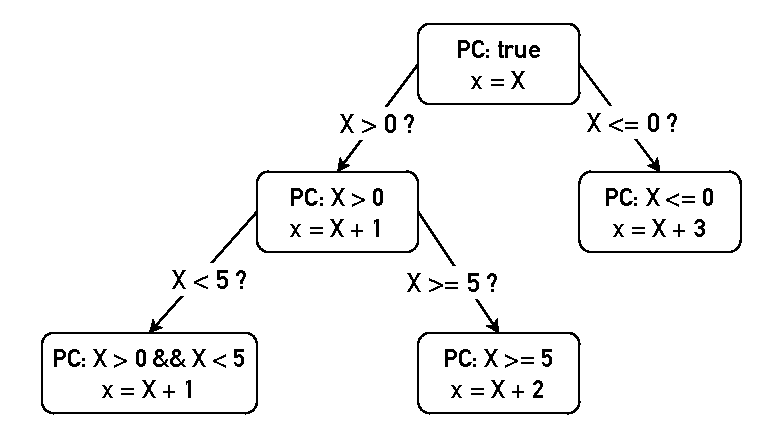
\includegraphics[height=%
            0.6\textheight]{../res/diagram-symexec}
        \end{column}
    \end{columns}
\end{frame}

\begin{frame}{Symbolic execution in Kratos}
    Kratos can, therefore:

    \begin{itemize}
        \item \textbf{Check path feasibility}: Cut out exploration on unreachable path constraints.

        \item \textbf{Generate inputs}: If a path constraint is satisfiable, the solver provides test assignments to symbolic inputs that satisfies the constraints.

        \item \textbf{Check properties}: In the same way, it can describe a violation in the validity of the assertion, providing a counterexample.
    \end{itemize}

    Resulting in a systematic exploration of the program's behavior and related properties.
\end{frame}

\section{Commutativity of Reducers}

\begin{frame}{The Map-Reduce programming model}
    The \textbf{Map-Reduce} programming paradigm is a high-level abstraction used in the design of functional programming algorithms and distributed systems.

    \bigskip

    The computation is split in two phases:
    \begin{itemize}
        \item \textbf{Map}: individual elements in the domain are reorganized in a new output format.

        \item \textbf{Reduce}: a functional transformation is applied to matching entries.
    \end{itemize}

    \begin{center}
        \includegraphics[height=%
        0.55\textheight]{../res/map-reduce}
    \end{center}
\end{frame}

\begin{frame}[fragile]{Commutativity of Reducers}
    \begin{block}{C implementation}
            \begin{minted}[fontsize=\footnotesize]{C}
int rangesum(int x[N]) {
    int i, cnt = 0;
    long long ret = 0;

    // sum up array values
    for (i = 0; i < N; i++) {
        // a bug! only the second half is summed up...
        if (i > N / 2) {
            ret = ret + x[i];
            cnt = cnt + 1;
        }
    }

    // standard average
    if (cnt != 0)
        return ret / cnt;
    else
        return 0;
}
            \end{minted}
    \end{block}
\end{frame}

\begin{frame}[fragile]{Commutativity of Reducers}
    \begin{columns}
        \begin{column}{0.45\textwidth}
            \begin{block}{A simple testing strategy}
                    \begin{minted}[fontsize=\footnotesize]{C}
int main() {
    // array size
    N = __VERIFIER_nondet_int();
    if (N > 1) {
        int x[N], temp, ret1, ret2, ret3;
        // initialize the array
        init_nondet(x);

        // base sum
        ret1 = rangesum(x);

        // swap x[0] and x[1]
        temp = x[0];
        x[0] = x[1];
        x[1] = temp;
        ret2 = rangesum(x);
                    \end{minted}
            \end{block}
        \end{column}
        \begin{column}{0.55\textwidth}
            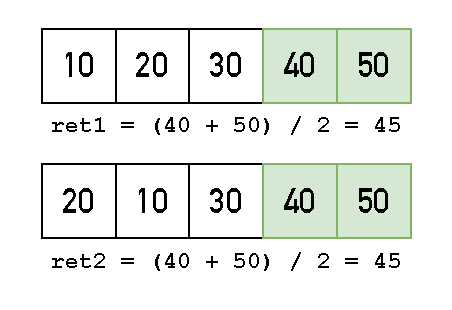
\includegraphics[height=%
            0.55\textheight]{../res/rangesum-ret1-2}
        \end{column}
    \end{columns}
\end{frame}

\begin{frame}[fragile]{Commutativity of Reducers}
    \begin{columns}
        \begin{column}{0.48\textwidth}
            \begin{block}{A simple testing strategy}
                    \begin{minted}[fontsize=\footnotesize]{C}
        // shift left (circularly)
        temp = x[0];
        for (int i = 0; i < N - 1; i++) {
            x[i] = x[i + 1];
        }
        x[N - 1] = temp;
        ret3 = rangesum(x);

        // compare results
        if (ret1 != ret2 || ret1 != ret3) {
            reach_error();
        }
    }
    return 1;
}
                    \end{minted}
            \end{block}
        \end{column}
        \begin{column}{0.55\textwidth}
            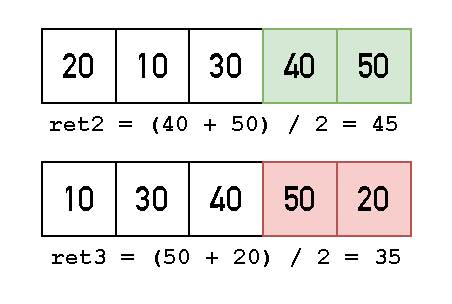
\includegraphics[height=%
            0.55\textheight]{../res/rangesum-ret3}
        \end{column}
    \end{columns}
\end{frame}

\begin{frame}[fragile]{Commutativity of Reducers}
    Let's apply \textbf{symbolic execution} to our example:

    \begin{block}{Linux shell command}
            \begin{minted}{bash}
python /kratos/tools/c2kratos.py
    --svcomp --svcomp-spec properties/unreach-call.prp
        rangesum.c | kratos -stage=symexec -error_id=reach_error
            \end{minted}
    \end{block}

    \bigskip

    \pause

    The wrapper makes the generation of \textbf{counterexamples} easier:

    \begin{block}{Linux shell command}
            \begin{minted}{bash}
python kratos-svcomp.py rangesum.c --cex
            \end{minted}
    \end{block}
\end{frame}

\begin{frame}[fragile]{Commutativity of Reducers}
    \begin{block}{Kratos output}
            \begin{minted}[fontsize=\footnotesize]{text}
-----------------------------------------------------------------------------
translating input C program to k2
-----------------------------------------------------------------------------
translation_time = 1.609
-----------------------------------------------------------------------------
running kratos with configuration: symexec
-----------------------------------------------------------------------------
parsing... done (0.019)
flattening... done (0.006)
building control-flow graph... done (0.004)
performing symbolic execution...
Counterexample trace
    ...
 done (3.717)

Symbolic execution statistics:
    ...
Global statistics:
    ...

unsafe
            \end{minted}
    \end{block}
\end{frame}

\section{Additional functionalities and intermediate representations}

\begin{frame}[fragile]{Intermediate stages}
    The intermediate stage of Kratos processing can be dumped: some of them are \textbf{proprietary}.

    \smallskip

    Others, like the CFG, can be analyzed with \href{https://dreampuf.github.io/GraphvizOnline/}{standard diagram drawing software}.

    \begin{columns}
        \begin{column}{0.35\textwidth}
            \begin{block}{Linux shell command}
                    \begin{minted}[fontsize=\footnotesize]{bash}
kratos -stage=mc
  -intermediate_output_dir=.
  -dump_intermediate_stages=true
  example.k2
                    \end{minted}
            \end{block}

            \pause

            \begin{block}{Kratos output}
                    \begin{minted}[fontsize=\tiny]{text}
parsing... done (0.028)
writing to ./parsed.k2
flattening... done (0.007)
writing to ./flattened.k2
inlining functions... done (0.007)
flattening after inlining... done (0.000)
writing to ./inlined.k2
building control-flow graph... done (0.007)
writing to ./cfg.dot
writing to ./bbcfg.dot
writing to ./cfg.k2
encoding into transition system... done (0.055)
writing to ./ts.vmt
                    \end{minted}
            \end{block}
        \end{column}

        \pause

        \begin{column}{0.65\textwidth}
            \vspace{0.5cm}
            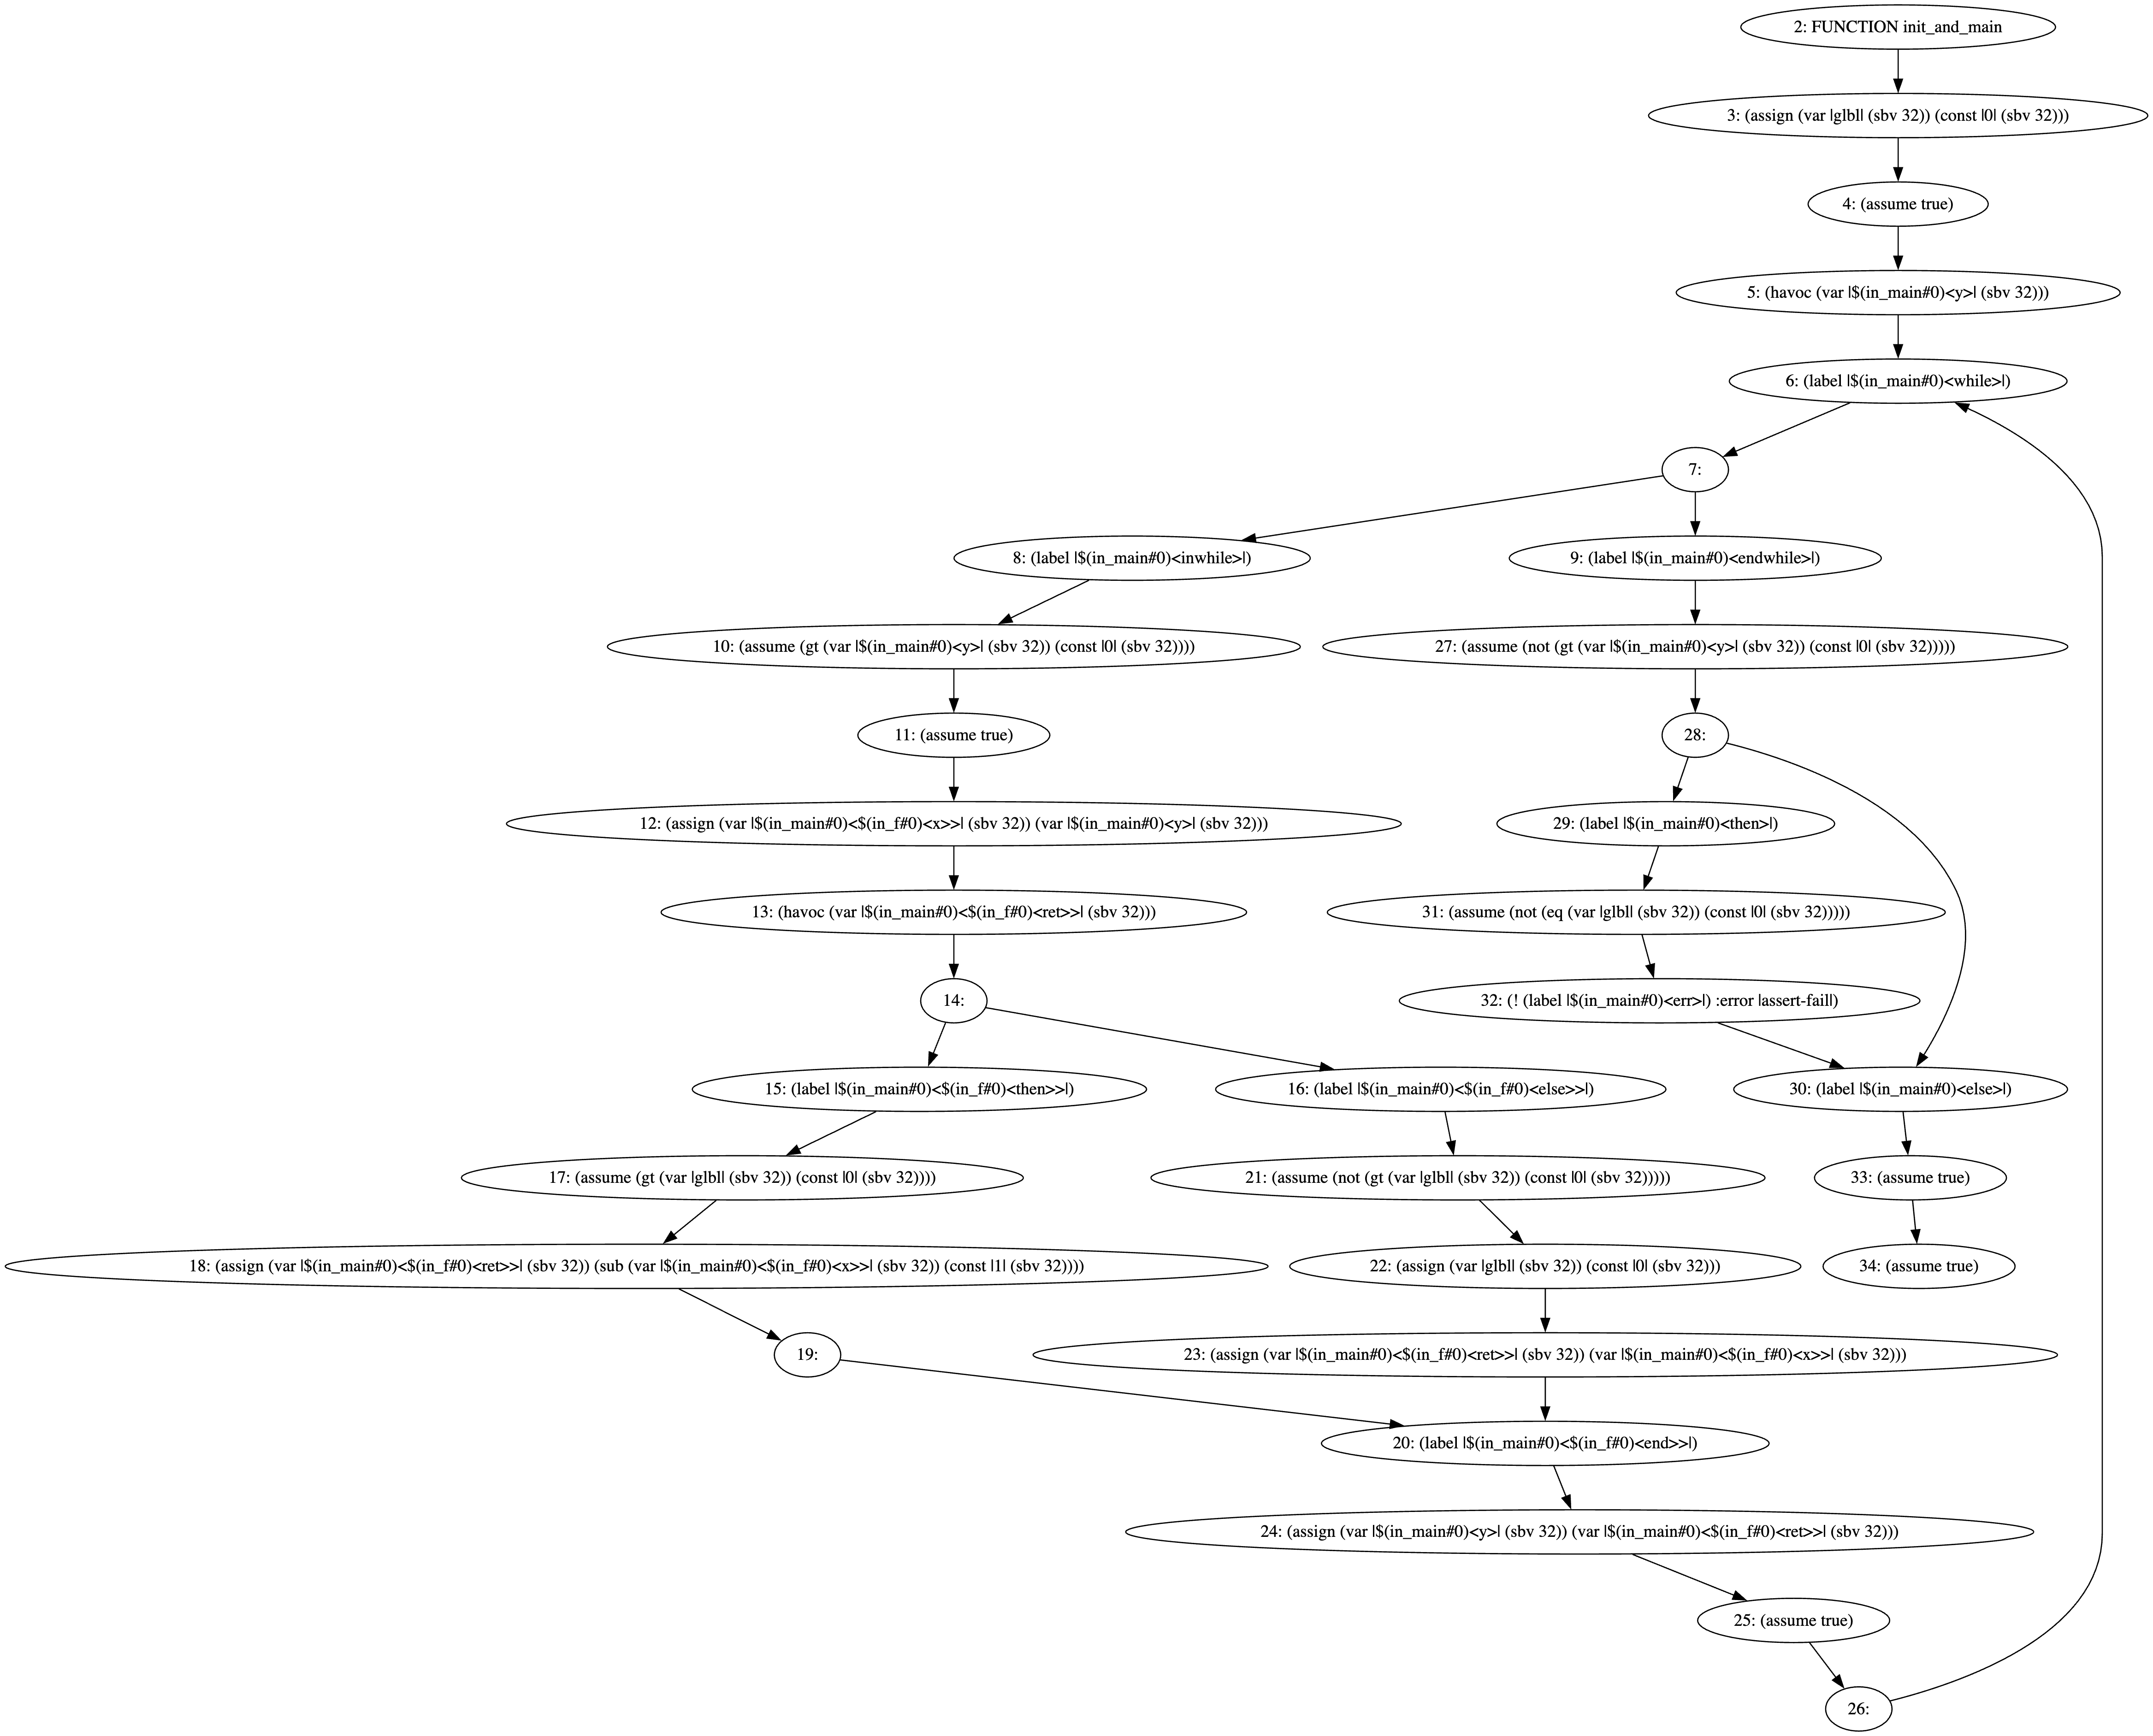
\includegraphics[height=%
            0.80\textheight]{../res/cfg}
        \end{column}
    \end{columns}
\end{frame}

\begin{frame}[fragile]{Interactive simulation: a first debugging technique}
    In Kratos, \textbf{interactive simulation} is a technique that aims at providing a first debugging end-point, by imposing \textbf{variable values, function returns and branches outcomes}.

    \smallskip

    Execution ends when an assumption is violated.

    \begin{block}{Linux shell command}
            \begin{minted}{bash}
kratos -stage=sim ./example.k2
            \end{minted}
    \end{block}
\end{frame}

\begin{frame}[fragile]{Interactive simulation: a first debugging technique}
    \begin{block}{Kratos output}
            \begin{minted}[fontsize=\tiny]{text}
parsing... done (0.022)
flattening... done (0.006)
inlining functions... done (0.005)
flattening after inlining... done (0.000)
building control-flow graph... done (0.011)
Enter input value for (var |glbl| (sbv 32)) (use ? for a random value)

0

executing statement: (assign (var |glbl| (sbv 32)) (const |0| (sbv 32)))
executing statement: (assume true)
executing statement: (havoc (var |$(in_main#0)<y>| (sbv 32)))
Enter input value for (var |$(in_main#0)<y>| (sbv 32)) (use ? for a random value)

1

executing statement: (label |$(in_main#0)<while>|)
Enter target value for (jump (label |$(in_main#0)<inwhile>|) (label |$(in_main#0)<endwhile>|)) (use ? for a random value)
$(in_main#0)<inwhile>
executing statement: (label |$(in_main#0)<inwhile>|)
executing statement: (assume (gt (var |$(in_main#0)<y>| (sbv 32)) (const |0| (sbv 32))))
executing statement: (assume true)
executing statement: (assign (var |$(in_main#0)<$(in_f#0)<x>>| (sbv 32)) (var |$(in_main#0)<y>| (sbv 32)))
executing statement: (havoc (var |$(in_main#0)<$(in_f#0)<ret>>| (sbv 32)))
Enter input value for (var |$(in_main#0)<$(in_f#0)<ret>>| (sbv 32)) (use ? for a random value)

1

Enter target value for (jump (label |$(in_main#0)<$(in_f#0)<then>>|) (label |$(in_main#0)<$(in_f#0)<else>>|)) (use ? for random value)

$(in_main#0)<$(in_f#0)<else>>
            \end{minted}
    \end{block}
\end{frame}

\begin{frame}[fragile]{Interactive simulation: a first debugging technique}
    \begin{block}{Kratos output}
            \begin{minted}[fontsize=\tiny]{text}
executing statement: (label |$(in_main#0)<$(in_f#0)<else>>|)
executing statement: (assume (not (gt (var |glbl| (sbv 32)) (const |0| (sbv 32)))))
executing statement: (assign (var |glbl| (sbv 32)) (const |0| (sbv 32)))
executing statement: (assign (var |$(in_main#0)<$(in_f#0)<ret>>| (sbv 32)) (var |$(in_main#0)<$(in_f#0)<x>>| (sbv 32)))
executing statement: (label |$(in_main#0)<$(in_f#0)<end>>|)
executing statement: (assign (var |$(in_main#0)<y>| (sbv 32)) (var |$(in_main#0)<$(in_f#0)<ret>>| (sbv 32)))
executing statement: (assume true)
executing statement: (label |$(in_main#0)<while>|)
Enter target value for (jump (label |$(in_main#0)<inwhile>|) (label |$(in_main#0)<endwhile>|)) (use ? for a random value)

$(in_main#0)<inwhile>

executing statement: (label |$(in_main#0)<inwhile>|)
executing statement: (assume (gt (var |$(in_main#0)<y>| (sbv 32)) (const |0| (sbv 32))))
executing statement: (assume true)
executing statement: (assign (var |$(in_main#0)<$(in_f#0)<x>>| (sbv 32)) (var |$(in_main#0)<y>| (sbv 32)))
executing statement: (havoc (var |$(in_main#0)<$(in_f#0)<ret>>| (sbv 32)))
Enter input value for (var |$(in_main#0)<$(in_f#0)<ret>>| (sbv 32)) (use ? for a random value)

1

Enter target value for (jump (label |$(in_main#0)<$(in_f#0)<then>>|) (label |$(in_main#0)<$(in_f#0)<else>>|)) (use ? for random value)

$(in_main#0)<$(in_f#0)<else>>

executing statement: (label |$(in_main#0)<$(in_f#0)<else>>|)
executing statement: (assume (not (gt (var |glbl| (sbv 32)) (const |0| (sbv 32)))))
executing statement: (assign (var |glbl| (sbv 32)) (const |0| (sbv 32)))
executing statement: (assign (var |$(in_main#0)<$(in_f#0)<ret>>| (sbv 32)) (var |$(in_main#0)<$(in_f#0)<x>>| (sbv 32)))
executing statement: (label |$(in_main#0)<$(in_f#0)<end>>|)
executing statement: (assign (var |$(in_main#0)<y>| (sbv 32)) (var |$(in_main#0)<$(in_f#0)<ret>>| (sbv 32)))
executing statement: (assume true)
executing statement: (label |$(in_main#0)<while>|)
            \end{minted}
    \end{block}
\end{frame}

\begin{frame}{Overall architecture}
    \begin{center}
        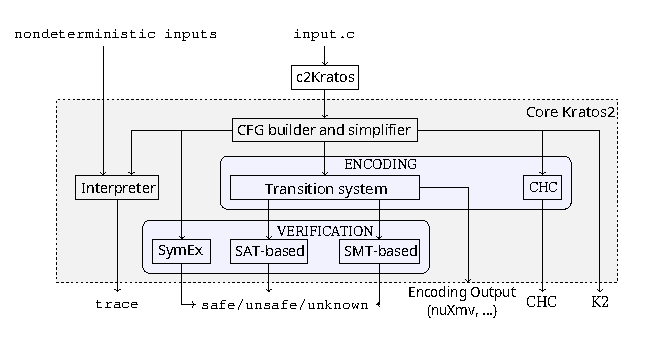
\includegraphics[height=%
        0.85\textheight]{../res/architecture-paper}
    \end{center}
\end{frame}

\section{Applications and practical real-world implementations}

\begin{frame}{AUTOSAR and the framework EVA}
    AUTOSAR (AUTomotive Open System ARchitecture) is a worldwide consortium of car manufacturers and component or service providers in the \textbf{automotive domain}, with the main goal of providing a standardized software architecture for the development and deployment of software components.

    \bigskip

    AUTOSAR wants to develop a platform for software development which ensures \textbf{safety}.

    \bigskip

    This platform is complemented by traditional V\&V (\textbf{Verification and Validation}) techniques.
\end{frame}

\begin{frame}{AUTOSAR and the framework EVA}
    AUTOSAR found a Solution in \textbf{EVA}, a framework for the \textbf{integration} of modern verification tools.

    \smallskip

    Main characteristics:

    \begin{itemize}
        \item Automatic end-to-end verification of \textbf{system-level properties}.
        \item Combines software model checking techniques with a \textbf{contract-based analysis} for verifying their correct composition.
        \item Implements all the features required for \textbf{usability} in a typical industrial context.
        \item Includes a \textbf{frontend} for the AUTOSAR's development environment.
    \end{itemize}
\end{frame}

\begin{frame}{AUTOSAR and the framework EVA}
    Arrows represent the flow of data: the input ones are the \textbf{Require Ports} and output ones are \textbf{Provide Ports}.

    \begin{center}
        \includegraphics[height=%
        0.40\textheight]{../res/AUTOSARModel}
    \end{center}

    The set of properties in AUTOSAR's environment is defined in simple Linear Temporal Logic (\textbf{LTL}) through predicates called \textbf{Contracts}.

    \begin{center}
        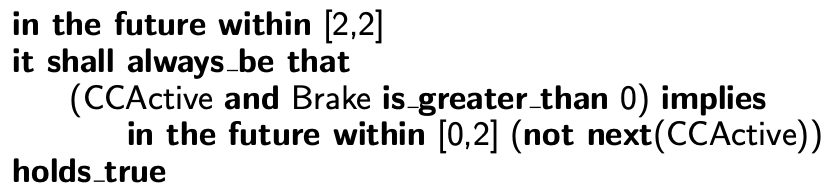
\includegraphics[height=%
        0.25\textheight]{../res/AUTOSARLogic}
    \end{center}
\end{frame}

\begin{frame}{Model checking in the automotive sector}
    Automated driving functions are among the \textbf{most critical software components} to develop.

    \smallskip

    Before deployment in real vehicles, they must be proven \textbf{safe} for both regulatory and traffic compliance.

    \bigskip

    Despite the coverage that can be reached with huge numbers of test drives, \textbf{corner cases} are possible and potential logic errors must be found as early as possible.

    \bigskip

    Due to time-to-delivery constraints, the V\&V activities which mainly involve model checking of infinite-state transition systems are supposed to proceed \textbf{in parallel} with the development.
\end{frame}

\begin{frame}{Model checking in the automotive sector}
    The main challenge is to \textbf{automate} V\&V process to increase efficiency and effectiveness in \textbf{edge case} discovery and \textbf{logical violation} during the development phase of an autonomous agent.

    \bigskip

    Kratos implements effective model checking engines that are being incrementally integrated in development process.

    \bigskip

    For example, it has been deployed in the \textbf{Behaviour Planner}, the portion of the agent's code that decides the rules to adopt given a set of inputs from the sensors (whether to brake, accelerate, turn left/right, \ldots).
\end{frame}

\begin{frame}{Model checking in the automotive sector}
    \begin{center}
        \includegraphics[height=%
        0.85\textheight]{../res/AutomotiveWorkflow}
    \end{center}
\end{frame}

\section{Demo}

\begin{frame}[fragile]{Introduction to the demo: Even or Odd? A recursive case}
    \begin{columns}
        \begin{column}{0.55\textwidth}
            \vspace{-0.5cm}
            \begin{block}{C implementation}
                    \begin{minted}[fontsize=\footnotesize]{C}
// returns 1 if the input n is odd
int isOdd(int n) {
    if (n == 0) {
        return 0;
    } else if (n == 1) {
        return 1;
    } else {
        return isEven(n - 1);
    }
}

// returns 1 if the input n is even
int isEven(int n) {
    if (n == 0) {
        return 1;
    } else if (n == 1) {
        return 0;
    } else {
        return isOdd(n - 1);
    }
}
                    \end{minted}
            \end{block}
        \end{column}
        \begin{column}{0.40\textwidth}
            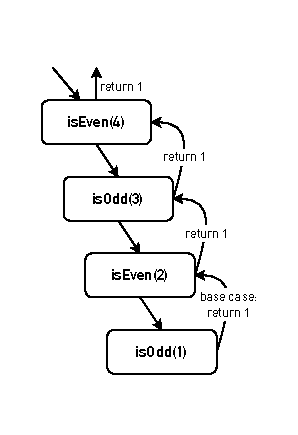
\includegraphics[width=%
            0.65\textheight]{../res/diagram-parity}
        \end{column}
    \end{columns}
\end{frame}

\begin{frame}{Demo}
    \begin{center}
        {\LARGE Time for the demo!}
    \end{center}
\end{frame}

\begin{frame}[fragile]{Even or Odd? A recursive case}
    \begin{block}{C implementation}
            \begin{minted}[fontsize=\footnotesize]{C}
int main() {
    int n = __VERIFIER_nondet_int();
    if (n < 0 || n > 400) return 0;

    int result = isEven(n);  // 1 if even, 0 if odd
    int mod = n % 2;         // 0 if even, 1 if odd

    if (result < 0 || result == mod) {
        return 0;
    } else {
    // our case
    ERROR: {
        reach_error();
        abort();
    }
    }
}
            \end{minted}
    \end{block}

    \pause

    \begin{block}{Linux shell command}
            \begin{minted}{bash}
python kratos-svcomp.py evenodd.c --cex
            \end{minted}
    \end{block}
\end{frame}

\begin{frame}[fragile]{Even or Odd? A recursive case}
    \begin{block}{Kratos output}
            \begin{minted}[fontsize=\footnotesize]{text}
-----------------------------------------------------------------------------
translating input C program to k2
-----------------------------------------------------------------------------
translation_time = 0.147
-----------------------------------------------------------------------------
running kratos with configuration: symexec
-----------------------------------------------------------------------------
parsing... done (0.015)
flattening... done (0.006)
building control-flow graph... done (0.002)
performing symbolic execution...
Counterexample trace
    ...
 done (0.064)

Symbolic execution statistics:
    ...
Global statistics:
    ...

unsafe
            \end{minted}
    \end{block}
\end{frame}

\begin{frame}[fragile]{Even or Odd? A recursive case}
    \begin{block}{Let's fix it!}
            \begin{minted}[fontsize=\footnotesize]{C}
int main() {
    ...

    int result = isOdd(n);  // 0 if even, 1 if odd
    int mod = n % 2;        // 0 if even, 1 if odd

    ...
}
            \end{minted}
    \end{block}

    \pause

    \begin{block}{Linux shell command}
            \begin{minted}{bash}
python kratos-svcomp.py evenodd.c
            \end{minted}
    \end{block}
\end{frame}

\begin{frame}[fragile]{Even or Odd? A recursive case}
    \begin{block}{Kratos output}
            \begin{minted}[fontsize=\footnotesize]{text}
-----------------------------------------------------------------------------
translating input C program to k2
-----------------------------------------------------------------------------
translation_time = 0.239
-----------------------------------------------------------------------------
running kratos with configuration: symexec
options: -stage=symexec -error_id=reach_error -symexec_iterative=true -symexec_max_depth=0
-----------------------------------------------------------------------------
parsing... done (0.015)
flattening... done (0.005)
building control-flow graph... done (0.003)
performing symbolic execution...
 done (28.722)

Symbolic execution statistics:
  ...

Global statistics:
  ...

safe
            \end{minted}
    \end{block}
\end{frame}

\begin{frame}[fragile]{The Kratos SV-COMP automated wrapper: a brief overview}
    \begin{block}{Python implementation}
            \begin{minted}[fontsize=\tiny]{C}
#!/usr/bin/env python

import os, sys, argparse
import tempfile
import shutil
import c2kratos.main
import kratos
import subprocess
import time

_common_mc_opts = "-stage=mc -inline_max_depth_add_check=true -propagate_constants=maps -remove_const_maps=true -apply_slicing=true"

configs = {
    "bmc": _common_mc_opts + " -model_checking_engine=bmc",
    "msatic3": _common_mc_opts
    + " -model_checking_engine=msatic3 -model_checking_invert_ts=true",
    "symexec": "-stage=symexec -error_id=reach_error -symexec_iterative=true -symexec_max_depth=0",
    "bitprophic3": _common_mc_opts + " -model_checking_engine=btoric3abs",
}

# format is: (name, time limit in seconds)
configorder = [
    ("symexec", 240),
    ("msatic3", 450),
    ("bitprophic3", 600),
    ("bmc", -1),
    # run symex again if other engines fail due to unsupported recursion
    ("symexec", -1),
    # Skipped configurations...
    ("msatic3", -1),
    ("bitprophic3", -1),
]

spec = "CHECK( init(main()), LTL(G ! call(reach_error())) )"
            \end{minted}
    \end{block}
\end{frame}

\begin{frame}[fragile]{The Kratos SV-COMP automated wrapper: a brief overview}
    \begin{block}{Python implementation}
            \begin{minted}[fontsize=\tiny]{C}
def c_to_k2(opts, tempdir):
    specfile = os.path.join(tempdir, "spec.prp")
    with open(specfile, "w") as out:
        out.write(spec)
    filename = os.path.join(tempdir, "program.k2")
    inputfile = opts.inputfile

    if opts.prefer_unprocessed:
        benchname, ext = os.path.splitext(inputfile)
        unprocessed = benchname + ".c"
        path, benchmark = os.path.split(unprocessed)
        path, family = os.path.split(path)
        if ext == ".i" and os.path.exists(unprocessed):
            print("Preferring unprocessed", unprocessed, file=sys.stderr)
            inputfile = unprocessed

    frontend_opts = ["--svcomp-spec", specfile, "--output", filename, inputfile]
    c2kratos.main.main(c2kratos.main.getopts(frontend_opts))
    return filename

def getopts():
    p = argparse.ArgumentParser()
    p.add_argument("inputfile")
    p.add_argument("--dump-k2")
    p.add_argument("--cex", action="store_true")
    p.add_argument("--translate-only", action="store_true")
    p.add_argument("--prefer-unprocessed", action="store_true")
    p.add_argument("--single-config")
    return p.parse_args()

def main():
    ...
            \end{minted}
    \end{block}
\end{frame}

\begin{frame}[fragile]{The Bubble Sorting algorithm: a development companion}
    \begin{block}{C implementation}
            \begin{minted}[fontsize=\footnotesize]{C}
// Limited for performance reasons...
#define N 5

int main() {
    int a[N];
    for (int j = 0; j < N; j++) {
        a[j] = __VERIFIER_nondet_int();
    }

    int swapped = 1;
    while (swapped) {
        swapped = 0;
        for (int i = 1; i < N; i++) {
            if (a[i - 1] > a[i]) {
                int t = a[i];
                a[i] = a[i - 1];
                a[i - 1] = t;
                swapped = 1;
            }
        }
    }
            \end{minted}
    \end{block}
\end{frame}

\begin{frame}[fragile]{The Bubble Sorting algorithm: a development companion}
    \begin{block}{C implementation}
            \begin{minted}[fontsize=\footnotesize]{C}
    int x, y;
    for (x = 0; x < N; x++) {
        for (y = x + 1; y < N; y++) {
            // multiple assertions!
            __VERIFIER_assert(a[x] <= a[y]);
        }
    }
    return 0;
}
            \end{minted}
    \end{block}

    \pause

    \begin{block}{Linux shell command}
            \begin{minted}{bash}
python kratos-svcomp.py bubblesort.c
            \end{minted}
    \end{block}
\end{frame}

\begin{frame}[fragile]{The Bubble Sorting algorithm: a development companion}
    \begin{block}{Kratos output}
            \begin{minted}[fontsize=\footnotesize]{text}
-----------------------------------------------------------------------------
translating input C program to k2
-----------------------------------------------------------------------------
translation_time = 0.136
-----------------------------------------------------------------------------
running kratos with configuration: symexec
-----------------------------------------------------------------------------
parsing... done (0.014)
flattening... done (0.004)
building control-flow graph... done (0.002)
performing symbolic execution...
 done (3.838)

Symbolic execution statistics:
  ...

Global statistics:
  ...

safe
            \end{minted}
    \end{block}
\end{frame}

\section{Conclusions and considerations}

\begin{frame}{Conclusions and considerations}
    \begin{columns}
        \begin{column}{0.47\textwidth}
            \begin{block}{Strengths}
                \begin{itemize}
                    \item Very precise translation engine.
                    \item Efficient model checking and symbolic execution models and algorithms.
                    \item Light on system resources.
                \end{itemize}
            \end{block}
        \end{column}
        \begin{column}{0.50\textwidth}
            \begin{block}{Weaknesses}
                \begin{itemize}
                    \item Poor documentation and distribution management.
                    \item Explicitly scoped only for research and evaluation.
                    \item Optimized on specific use-cases.
                \end{itemize}
            \end{block}
        \end{column}
    \end{columns}

\end{frame}

\begin{frame}{Bibliography}
    \begin{block}{References}
        {\footnotesize
            \begin{thebibliography}{9}
                \bibitem{1} [1] Fondazione Bruno Kessler (2023), \href{https://kratos.fbk.eu/documentation.html}{Kratos 2: documentation}.
                \bibitem{2} [2] Alberto Griggio and Martin Jonás (2023), \href{https://es-static.fbk.eu/people/griggio/papers/cav23a.pdf}{Kratos2: an SMT-Based Model Checker for Imperative Programs}.
                \bibitem{3} [3] Alberto Griggio and Martin Jonás (2023), \href{https://doi.org/10.5281/zenodo.7876934}{Artifact for Kratos2: an SMT-Based Model Checker for Imperative Programs (experimental evaluation)}.
                \bibitem{4} [4] AA. VV. (2023), \href{https://es-static.fbk.eu/people/griggio/papers/tacas23.pdf}{EVA: a Tool for the Compositional Verification of AUTOSAR Models}.
                \bibitem{5} [5] AA. VV. (2024), \href{https://es-static.fbk.eu/people/griggio/papers/tacas24.pdf}{Towards Safe Autonomous Driving: Model Checking a Behavior Planner during Development}.
                \bibitem{6} [6] Software and Computational Systems Lab and AA. VV. at LMU Munich, \href{https://gitlab.com/sosy-lab/benchmarking/sv-benchmarks/}{SV-COMP: Collection of Verification Tasks}.
                \bibitem{7} [7] Alberto Griggio and Marco Roveri (2015), \href{https://es-static.fbk.eu/people/griggio/papers/tcad15.pdf}{Comparing Different Variants of the IC3 Algorithm for Hardware Model Checking}.
                \bibitem{8} [8] Sean Eron Anderson (2005), \href{https://graphics.stanford.edu/~seander/bithacks.html}{Bit manipulation hacks: modulus division without a division operator}.
            \end{thebibliography}
        }
    \end{block}
\end{frame}
\end{document}